% ===================================================================
%  Week 1 — Digital Images & the Pipeline
%  Compile: pdflatex -interaction=nonstopmode slides.tex  (twice)
% ===================================================================
\documentclass[10pt,aspectratio=169]{beamer}
% ===================================================================
%  Shared Beamer preamble for "Practical Image Processing"
%  English slides. Compile with pdfLaTeX.
% ===================================================================

\usetheme{metropolis}
\usepackage[T1]{fontenc}
\usepackage[utf8]{inputenc}
\usepackage{lmodern}
\usepackage{listings}
\usepackage{tcolorbox}
\usepackage{fontawesome5}
\usepackage{booktabs}
\usepackage{amsmath,amssymb}
\usepackage{tikz}
\usepackage{pgfplots}
\pgfplotsset{compat=1.17}
\usetikzlibrary{arrows.meta,positioning,shapes.geometric,fit,backgrounds,matrix}
\tcbuselibrary{skins,breakable}

% ---- Palette --------------------------------------------------------
\definecolor{coursePrimary}{HTML}{1B4965}   % deep blue
\definecolor{courseAccent}{HTML}{E76F51}    % coral
\definecolor{courseGood}{HTML}{2A9D8F}      % teal
\definecolor{courseBad}{HTML}{C0392B}       % red
\definecolor{courseInfo}{HTML}{2980B9}      % blue
\definecolor{codeBg}{HTML}{F5F6FA}
\definecolor{codeKw}{HTML}{8E44AD}
\definecolor{codeStr}{HTML}{2A9D8F}
\definecolor{codeCom}{HTML}{7F8C8D}

\setbeamercolor{frametitle}{bg=coursePrimary}
\setbeamercolor{progress bar}{fg=courseAccent}
\setbeamercolor{alerted text}{fg=courseAccent}
\metroset{block=fill,sectionpage=progressbar,numbering=fraction}

% ---- Code listings (Python is built into listings) -----------------
\lstdefinestyle{course}{
  backgroundcolor=\color{codeBg},
  basicstyle=\ttfamily\scriptsize,
  keywordstyle=\color{codeKw}\bfseries,
  stringstyle=\color{codeStr},
  commentstyle=\color{codeCom}\itshape,
  numberstyle=\tiny\color{codeCom},
  numbers=left, numbersep=6pt,
  showstringspaces=false, breaklines=true, breakatwhitespace=true,
  tabsize=4, columns=fullflexible,
  frame=single, framesep=4pt, rulecolor=\color{gray!30},
  keepspaces=true, upquote=true, language=Python,
}
\lstset{style=course}
\lstdefinelanguage{bash}{
  keywords={cd,pip,python,venv,source,import}, sensitive=true,
  morecomment=[l]{\#}, morestring=[b]', morestring=[b]",
}

% ---- Reusable callout boxes ----------------------------------------
\newtcolorbox{goodbox}[1][Good practice]{colback=courseGood!8,colframe=courseGood,
  fonttitle=\bfseries,title={\faCheck~#1},boxrule=0.6pt,left=4pt,right=4pt,top=3pt,bottom=3pt}
\newtcolorbox{badbox}[1][Pitfall]{colback=courseBad!8,colframe=courseBad,
  fonttitle=\bfseries,title={\faTimes~#1},boxrule=0.6pt,left=4pt,right=4pt,top=3pt,bottom=3pt}
\newtcolorbox{infobox}[1][Note]{colback=courseInfo!8,colframe=courseInfo,
  fonttitle=\bfseries,title={\faInfoCircle~#1},boxrule=0.6pt,left=4pt,right=4pt,top=3pt,bottom=3pt}
\newtcolorbox{mathbox}[1][Math]{colback=coursePrimary!6,colframe=coursePrimary,
  fonttitle=\bfseries,title={\faCalculator~#1},boxrule=0.6pt,left=4pt,right=4pt,top=3pt,bottom=3pt}

\newcommand{\keyidea}[1]{\begin{alertblock}{Key idea}#1\end{alertblock}}
\newcommand{\term}[1]{\textbf{\color{coursePrimary}#1}}
\newcommand{\code}[1]{\lstinline[basicstyle=\ttfamily\small]|#1|}

% ---- A helper to draw a small pixel grid, cells shaded by value ----
% \pixelgrid{ {10,20,120,200,240}, {30,60,130,180,230}, ... }
\newcommand{\pixelgrid}[1]{%
  \begin{tikzpicture}[font=\scriptsize,scale=0.6]
    \foreach \row [count=\ry] in {#1} {
      \foreach \val [count=\cx] in \row {
        \draw[gray,fill=coursePrimary!8] (\cx,-\ry) rectangle ++(1,-1);
        \node at (\cx+0.5,-\ry-0.5) {\val};
      }
    }
  \end{tikzpicture}}


\title{Digital Images \& the Pipeline}
\subtitle{Week 1 — What an image really is}
\author{Practical Image Processing}
\date{Lecture 1 \textbullet\ 60--70 min}

\begin{document}

\maketitle

\begin{frame}{Where this course is going}
  \begin{columns}[T]
    \begin{column}{0.56\textwidth}
      By the end you will build \alert{DocScan}: a photo of a document $\rightarrow$ a clean,
      deskewed, machine-readable scan, then read it with a small neural net.
      \begin{itemize}
        \item Tools: \term{Python + OpenCV + NumPy}.
        \item Weeks 1--11: classical image processing.
        \item Weeks 12--14: an introduction to deep learning for vision.
      \end{itemize}
    \end{column}
    \begin{column}{0.44\textwidth}
      \begin{alertblock}{The habit we build}
        Understand the pixels and the math \emph{first}; call the library second; reach for a
        neural net only when classical methods run out.
      \end{alertblock}
    \end{column}
  \end{columns}
\end{frame}

\begin{frame}{The image-processing pipeline}
  \begin{center}
  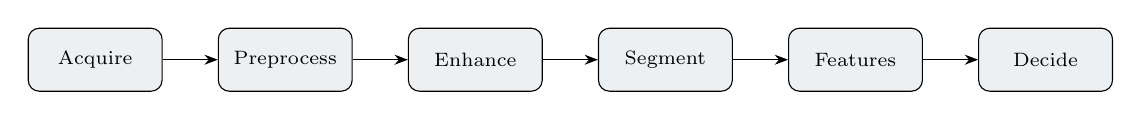
\begin{tikzpicture}[font=\scriptsize,>=Stealth,node distance=3mm and 7mm,
    b/.style={draw,rounded corners,fill=coursePrimary!8,minimum height=8mm,minimum width=17mm,align=center}]
    \node[b] (acq){Acquire};
    \node[b,right=of acq] (pre){Preprocess};
    \node[b,right=of pre] (enh){Enhance};
    \node[b,right=of enh] (seg){Segment};
    \node[b,right=of seg] (feat){Features};
    \node[b,right=of feat] (dec){Decide};
    \draw[->](acq)--(pre);\draw[->](pre)--(enh);\draw[->](enh)--(seg);\draw[->](seg)--(feat);\draw[->](feat)--(dec);
  \end{tikzpicture}
  \end{center}
  \keyidea{Every task in this course is some path through this pipeline. DocScan walks all of it.}
\end{frame}

\begin{frame}{Roadmap}\tableofcontents\end{frame}

% ==================================================================
\section{What is a digital image?}
% ==================================================================

\begin{frame}{An image is a function, sampled onto a grid}
  \begin{itemize}
    \item A continuous image is a function $f(x,y)$ = brightness at position $(x,y)$.
    \item A \term{digital} image samples it on a grid and rounds each value: \term{pixels}.
    \item A grayscale image is a 2D array; a color image is 3 such arrays (channels).
  \end{itemize}
  \begin{mathbox}
    $f(x,y)$, with $x=0\dots W{-}1$, $y=0\dots H{-}1$, and each value in $\{0,\dots,255\}$ (8-bit).
  \end{mathbox}
\end{frame}

\begin{frame}{Pixels are just numbers}
  \begin{columns}[T]
    \begin{column}{0.5\textwidth}
      A tiny 5$\times$5 patch of intensities:
      \begin{center}
      \pixelgrid{
        {10,20,120,200,240},
        {30,60,130,180,230},
        {50,90,150,190,220},
        {70,110,160,200,250},
        {90,130,170,210,255}
      }
      \end{center}
    \end{column}
    \begin{column}{0.5\textwidth}
      \begin{itemize}
        \item 0 = black, 255 = white, values between = gray.
        \item ``Processing'' an image = doing arithmetic on these numbers.
        \item There is no magic: every operation is math on an array.
      \end{itemize}
    \end{column}
  \end{columns}
\end{frame}

\begin{frame}{A real image from our dataset}
  \begin{columns}[T]
    \begin{column}{0.5\textwidth}
      \begin{center}
      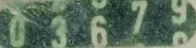
\includegraphics[width=\linewidth]{../assets/meter_bgr.png}\\[2pt]
      {\scriptsize original (color) — a water-meter numerator}
      \end{center}
    \end{column}
    \begin{column}{0.5\textwidth}
      \begin{center}
      
\includegraphics[width=\linewidth]{../assets/meter_gray.png}\\[2pt]
      {\scriptsize grayscale — one channel, same structure}
      \end{center}
    \end{column}
  \end{columns}
  \vspace{4pt}
  This 48$\times$196 crop is our running example. Reading these digits is exactly what the
  DocScan capstone builds toward. (Data: \code{E:/data/abfa\_image/numerators}.)
\end{frame}

\begin{frame}{Sampling: how finely we measure space}
  \begin{center}
  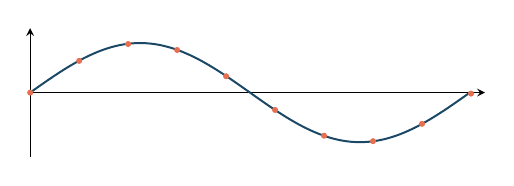
\begin{tikzpicture}[scale=0.9]
    \begin{axis}[width=8cm,height=3.4cm,ticks=none,axis lines=middle,
      xmin=0,xmax=6.5,ymin=-1.3,ymax=1.3,clip=false,font=\tiny]
      \addplot[coursePrimary,thick,domain=0:6.3,samples=100]{sin(deg(x))};
      \addplot[courseAccent,only marks,mark=*,mark size=1pt]
        coordinates{(0,0)(0.7,0.64)(1.4,0.98)(2.1,0.86)(2.8,0.33)(3.5,-0.35)(4.2,-0.87)(4.9,-0.98)(5.6,-0.63)(6.3,-0.02)};
    \end{axis}
  \end{tikzpicture}
  \end{center}
  \term{Sampling} = choosing grid points (resolution). Too few samples and detail is lost —
  or worse, faked (aliasing, deep dive). More pixels = more spatial detail, more data.
\end{frame}

\begin{frame}{Quantization: how finely we measure brightness}
  \begin{itemize}
    \item \term{Quantization} = rounding each sample to a finite set of levels (the bit depth).
    \item 8-bit = 256 levels (0--255); 1-bit = black/white; 16-bit = 65{,}536 (medical/RAW).
    \item Too few levels $\rightarrow$ visible \term{banding} in smooth gradients.
  \end{itemize}
  \begin{infobox}
    Resolution (sampling) and bit depth (quantization) are the two axes of ``how much image.''
  \end{infobox}
\end{frame}

\begin{frame}{Resolution, size, and memory}
  \begin{itemize}
    \item A $W\times H$ grayscale 8-bit image is $W\cdot H$ bytes; color is $3\times$ that.
    \item A 12-megapixel color photo $\approx$ 36\,MB \emph{uncompressed}.
    \item That's why formats compress — and why processing big images needs care (Week 11).
  \end{itemize}
  \keyidea{Know your image's shape and dtype before anything else: \code{img.shape}, \code{img.dtype}.}
\end{frame}

% ==================================================================
\section{Color}
% ==================================================================

\begin{frame}{Color: three numbers per pixel}
  \begin{itemize}
    \item \term{RGB}: red, green, blue channels; how screens emit light.
    \item A color pixel is a triple $(R,G,B)$, each 0--255.
    \item Grayscale collapses color to one intensity — often the first step (less data, same structure).
  \end{itemize}
  \begin{mathbox}
    Luminance: $Y = 0.299R + 0.587G + 0.114B$ — green dominates because our eyes do.
  \end{mathbox}
\end{frame}

\begin{frame}{Why convert to grayscale}
  \begin{itemize}
    \item Many operations (edges, thresholds) need intensity, not color — 1 channel, 3$\times$ less work.
    \item DocScan works mostly in grayscale; color returns only when it carries information.
    \item But grayscale \emph{discards} information — don't do it if hue matters (Week 8 color segmentation).
  \end{itemize}
  \begin{badbox}
    Averaging $(R+G+B)/3$ is a common shortcut — but the weighted luminance is perceptually correct.
  \end{badbox}
\end{frame}

\begin{frame}{Other color spaces, and why}
  \begin{center}
  \begin{tabular}{@{}lll@{}}
    \toprule
    \textbf{Space} & \textbf{Channels} & \textbf{Good for} \\
    \midrule
    RGB & red, green, blue & storage, display \\
    Grayscale & intensity & most classical processing \\
    HSV & hue, saturation, value & color-based selection (robust to lighting) \\
    Lab & lightness, a, b & perceptual distance, color correction \\
    \bottomrule
  \end{tabular}
  \end{center}
  \keyidea{Choosing the right color space can make a hard problem easy — e.g. ``find the red object'' is trivial in HSV, painful in RGB.}
\end{frame}

\begin{frame}{HSV intuition}
  \begin{itemize}
    \item \term{Hue}: which color (angle on the color wheel). \term{Saturation}: how vivid. \term{Value}: how bright.
    \item Separating color from brightness makes selection robust to shadows and lighting.
    \item ``All the red pixels'' = a hue range — one threshold, done.
  \end{itemize}
\end{frame}

% ==================================================================
\section{Images in code}
% ==================================================================

\begin{frame}[fragile]{An image is a NumPy array}
\begin{lstlisting}[language=Python]
import cv2, numpy as np
img = cv2.imread('page.jpg')          # BGR, shape (H, W, 3), dtype uint8
print(img.shape, img.dtype)           # e.g. (1200, 900, 3) uint8
gray = cv2.cvtColor(img, cv2.COLOR_BGR2GRAY)  # (H, W)
print(gray[0, 0])                     # a single pixel's intensity, 0..255
\end{lstlisting}
  \begin{badbox}[OpenCV gotcha]
    OpenCV loads images as \term{BGR}, not RGB. Forgetting this flips red and blue everywhere.
  \end{badbox}
\end{frame}

\begin{frame}[fragile]{Pixels, slices, and vectorized ops}
\begin{lstlisting}[language=Python]
h, w = gray.shape
roi = gray[100:200, 50:150]           # a rectangular region (a view)
gray[gray < 50] = 0                    # vectorized: threshold dark pixels to black
brighter = np.clip(gray.astype(int) + 40, 0, 255).astype(np.uint8)
\end{lstlisting}
  \begin{goodbox}
    Never loop over pixels in Python — it's 100$\times$ slower. Use NumPy vectorization / OpenCV.
  \end{goodbox}
\end{frame}

\begin{frame}[fragile]{Show and save}
\begin{lstlisting}[language=Python]
import matplotlib.pyplot as plt
plt.imshow(cv2.cvtColor(img, cv2.COLOR_BGR2RGB)); plt.axis('off'); plt.show()
cv2.imwrite('gray.png', gray)         # PNG = lossless; JPG would re-compress
\end{lstlisting}
  \begin{infobox}
    Convert BGR$\rightarrow$RGB before \code{plt.imshow}, or your colors look wrong.
  \end{infobox}
\end{frame}

\begin{frame}{The uint8 overflow trap — seen on real data}
  \begin{columns}[T]
    \begin{column}{0.5\textwidth}
      \begin{center}
      
\includegraphics[width=\linewidth]{../assets/meter_bright_ok.png}\\[2pt]
      {\scriptsize \code{+60} done right (clip): uniformly brighter}
      \end{center}
    \end{column}
    \begin{column}{0.5\textwidth}
      \begin{center}
      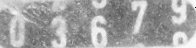
\includegraphics[width=\linewidth]{../assets/meter_bright_overflow.png}\\[2pt]
      {\scriptsize \code{+60} in uint8: bright pixels \emph{wrapped} to dark}
      \end{center}
    \end{column}
  \end{columns}
  \vspace{2pt}
  \begin{badbox}
    $200 + 100 = 44$, not 255. Cast to \code{int}, compute, \code{clip} to 0--255 — or use
    \code{cv2.add} (saturating). A ``brighten'' that darkens bright areas is this bug.
  \end{badbox}
\end{frame}

% ==================================================================
\section{In-class exercise}
% ==================================================================

\begin{frame}[fragile]{\faPen~In-class exercise (10 min)}
  \begin{infobox}[Predict, then run]
  \end{infobox}
\begin{lstlisting}[language=Python]
gray = np.array([[100, 150],[200, 250]], dtype=np.uint8)
a = gray + 60          # (1) what are the four values?
b = cv2.add(gray, 60)  # (2) and here?
c = gray.mean()        # (3) what does this represent?
\end{lstlisting}
  \begin{enumerate}
    \item Compute \code{a} by hand — watch the overflow. \quad 2. How does \code{b} differ?
    \item What is \code{c}, and what would a very low \code{c} tell you about the image?
  \end{enumerate}
\end{frame}

\begin{frame}{\faPen~Debrief}
  \begin{itemize}
    \item \code{a} = \code{[[160,210],[4,54]]} — 200+60 and 250+60 \emph{wrapped} (overflow).
    \item \code{b} = \code{[[160,210],[255,255]]} — \code{cv2.add} saturates (clamps to 255).
    \item \code{c} = mean intensity ($\approx$175); a very low mean means a mostly dark image (under-exposed).
  \end{itemize}
  \keyidea{The mean/histogram of an image tells you about exposure before you look at it — Week 2.}
\end{frame}

% ==================================================================
\section{Formats \& storage}
% ==================================================================

\begin{frame}{Image formats: lossless vs lossy}
  \begin{center}
  \begin{tabular}{@{}lll@{}}
    \toprule
    \textbf{Format} & \textbf{Compression} & \textbf{Use} \\
    \midrule
    PNG & lossless & masks, line art, intermediate results \\
    JPEG & lossy & photos; small files, but artifacts \\
    TIFF & lossless/none & archival, scientific, multi-page \\
    BMP/RAW & none & simplicity / sensor data \\
    \bottomrule
  \end{tabular}
  \end{center}
  \keyidea{Never save intermediate results as JPEG — its artifacts corrupt later processing.
  Use PNG until the very end.}
\end{frame}

\begin{frame}{JPEG artifacts matter for processing}
  \begin{itemize}
    \item JPEG discards high-frequency detail in 8$\times$8 blocks — invisible to you, poison to edge detection.
    \item Re-saving a JPEG repeatedly compounds the damage (generation loss).
    \item For DocScan, work from the least-compressed source you can get.
  \end{itemize}
\end{frame}

\begin{frame}{Bit depth \& dynamic range}
  \begin{itemize}
    \item 8-bit is fine for display; 12--16-bit sensors keep detail in shadows/highlights.
    \item \term{Dynamic range} = ratio of brightest to darkest a sensor can capture.
    \item HDR combines exposures to exceed a single sensor's range (beyond our scope, good to know).
  \end{itemize}
\end{frame}

% ==================================================================
\section{Deep dive: the imaging model}
% ==================================================================

\begin{frame}{Sampling theory \& aliasing}
  \begin{itemize}
    \item \term{Nyquist}: to capture detail at frequency $f$, sample at $>2f$. Under-sample and high frequencies masquerade as low ones.
    \item That's \term{aliasing}: moir\'e patterns, jagged edges, wagon-wheels spinning backwards.
    \item Fix: blur (low-pass) \emph{before} down-sampling — remove detail you can't represent (Week 3, 6).
  \end{itemize}
  \begin{badbox}
    Resizing an image down without blurring first creates aliasing artifacts that no later step can undo.
  \end{badbox}
\end{frame}

\begin{frame}{Gamma: pixels aren't linear light}
  \begin{itemize}
    \item Displays and files are \term{gamma-encoded}: pixel value $\ne$ linear light intensity.
    \item Storing perceptually (more codes for dark tones, where eyes are sensitive) saves bits.
    \item For \emph{correct} math (averaging, blending), sometimes linearize first — a common subtle bug.
  \end{itemize}
  \begin{mathbox}
    Encoded $\approx$ (linear)$^{1/\gamma}$, with $\gamma\approx 2.2$. We'll use gamma for contrast in Week 2.
  \end{mathbox}
\end{frame}

\begin{frame}{Where pixels come from}
  \begin{center}
  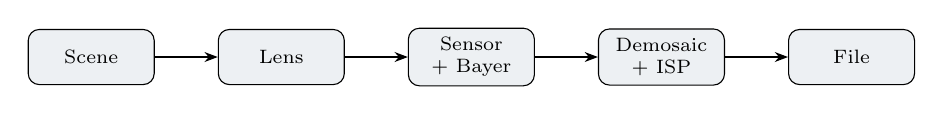
\begin{tikzpicture}[font=\scriptsize,>=Stealth,node distance=3mm and 8mm,
    b/.style={draw,rounded corners,fill=coursePrimary!8,minimum height=7mm,minimum width=16mm,align=center}]
    \node[b] (scene){Scene};
    \node[b,right=of scene] (lens){Lens};
    \node[b,right=of lens] (cfa){Sensor\\+ Bayer};
    \node[b,right=of cfa] (isp){Demosaic\\+ ISP};
    \node[b,right=of isp] (file){File};
    \draw[->](scene)--(lens);\draw[->](lens)--(cfa);\draw[->](cfa)--(isp);\draw[->](isp)--(file);
  \end{tikzpicture}
  \end{center}
  Real sensors capture one color per pixel (a \term{Bayer} mosaic) and interpolate the rest.
  Noise, blur, and color casts enter here — which is exactly what we clean up (Weeks 4, 2).
\end{frame}

\begin{frame}{Noise is physical, not a bug}
  \begin{itemize}
    \item Photon counting is random $\rightarrow$ shot noise; electronics add read noise.
    \item Low light / high ISO = more noise. It's the raw material Week 4 removes.
    \item Understanding \emph{where} noise comes from tells you \emph{how} to model and remove it.
  \end{itemize}
  \keyidea{Every artifact you'll fight — noise, blur, aliasing, color cast — has a physical origin in this pipeline.}
\end{frame}

\begin{frame}{Coordinates \& conventions}
  \begin{itemize}
    \item Images are indexed \code{[row, col]} = \code{[y, x]} — the \emph{opposite} of math $(x,y)$.
    \item Origin is top-left; $y$ increases \emph{downward}. This trips up everyone once.
    \item OpenCV points are \code{(x, y)}; NumPy indices are \code{[y, x]}. Keep them straight.
  \end{itemize}
  \begin{badbox}
    Swapping x and y is the \#1 beginner bug in image code. When something's transposed, check this first.
  \end{badbox}
\end{frame}

% ==================================================================
\section{Wrap-up}
% ==================================================================

\begin{frame}{What you should now be able to do}
  \begin{itemize}
    \item Explain sampling, quantization, resolution, and bit depth.
    \item Load an image, inspect its shape/dtype, convert color, slice regions — vectorized.
    \item Choose a color space and format for a task; avoid the uint8/BGR/xy traps.
    \item Name where noise, blur, and aliasing physically come from.
  \end{itemize}
\end{frame}

\begin{frame}{This week's deliverable}
  \begin{alertblock}{Due before Week 2 (see \code{project/})}
    \begin{enumerate}
      \item Load 3 images; print shape, dtype, min/max/mean; convert to grayscale and to HSV.
      \item Write a correct \code{brighten(img, k)} (no overflow) and compare to \code{cv2.add}.
      \item Take a phone photo of a document — your DocScan test image. Report its properties.
      \item Short note: for your photo, which stages of the pipeline will be hardest, and why?
    \end{enumerate}
  \end{alertblock}
\end{frame}

\begin{frame}[standout]
  An image is just numbers on a grid.\\[4pt]
  \normalsize Everything else in this course is arithmetic on those numbers.
\end{frame}

\end{document}
